\documentclass{es50report}

\usepackage{setspace}
\usepackage{palatino}

% \usepackage{url}
\usepackage{hyperref}
\usepackage{natbib}

\usepackage{graphicx}
\usepackage{caption}
\usepackage{subcaption}

\title{RetroBlue}
\projDescription{A Bluetooth-enabled vintage rotary phone that can be paired with a cell phone to make and receive calls.}
\authors{Kyle Solan, Michael Tingley, and Michael Traver}

\begin{document}
    \maketitlepage

    \begin{abstract}
        RetroBlue is a modern cell phone accessory with an old-timey feel. We took a vintage rotary phone, an Arduino board, and a Bluetooth chip and combined them to create RetroBlue, a fully functional Bluetooth accessory that can make, dial, and receive calls via a cell phone. A user simply pairs his or her cell phone with RetroBlue and all calls are then forwarded to the unit. We worked extensively to convert the antiquated circuitry within the phone to portable battery-powered components and developed custom code and circuitry to pass calls to and from the rotary phone's hardware.
    \end{abstract}
    \newpage

    \section{Introduction}
    TODO

    \section{Design}
        We had clear goals and objectives that guided much of the design process for our project. We wanted to emulate the experience of using a vintage rotary phone, but rotary phones often interface poorly with modern landlines, and furthermore, landlines are becoming less and less common altogether. So, we decided that a creating a desktop accessory that can pair with a cell phone via Bluetooth was the best way to achieve this.
        
        The Bluetooth standard includes many profiles, or specifications that define a certain type of wireless communication over a Bluetooth connection. The Hands-Free Profile (\url{http://en.wikipedia.org/wiki/Bluetooth_profile#Hands-Free_Profile_.28HFP.29}) allows a device to control a cell phone, including making and receiving calls and transmitting audio to and from the phone, and is commonly used in car Bluetooth accessories. This profile was a natural fit for our project, and we found a number of Bluetooth chips online that support HFP and provide a serial interface for communication.
        
        Traditional landline phones are made up of very simple hardware. The hardware itself is merely responsible for transmitting signals to the telephone exchange and interpreting and outputting signals it receives (such as a ring signal or an audio signal). All logic -- including detecting which number was dialed and routing a call -- is carried out by the service provider. Our system, in contrast, needs to be aware of its own state, interpret its own signals, and transmit all this information to the Bluetooth module via digital serial communication. For this we elected to use an Arduino board, which provides the ability to interface with our diverse set of components and to run our own event-handling logic.

        With this basic system in mind, we began our implementation process. Initially, we had the idea to use our Arduino as a simulated service provider and connect it directly to the phone's external data/power line. With this, we would not have needed to modify the phone's internal hardware. This situation, however, quickly proved impractical. Landline phones are meant to run on high voltage (50-90V), and much of the hardware is activated via large voltage fluctuations. This is poorly suited to our goal of having a free-standing portable accessory and would have required a lot of external circuitry to meet these power requirements. Instead, we found we could modernize the phone circuitry to run on a much lower voltage well-suited to battery power (3.3-5V) if we worked directly with each independent component within the phone.

        However, the electromagnetic coil that drives the ringer still requires a high voltage even when isolated. We decided to remove the original ringer components and replace them with a small solenoid that runs on 12-18V, suitable for battery power. The new solenoid still uses the original ringer bell, and it produces a good ring with a fraction of the power.

        With this initial hurdle overcome, we began by breaking the project up into independent circuits and components: the dialer, the ringer, the earpiece, the microphone, and the hook. We worked to implement circuits and test functionality for each of these components independently. Afterward, we connected each of them to the Arduino and Bluetooth module and wrote Arduino code to oversee the phone's global state and handle signals appropriately. After we achieved proper overall functionality, we consolidated these independent circuits into a single circuit operating on a single power source. The ringer solenoid does, however, require a higher voltage, which we provide with two 9V batteries wired in series.

    \section{Parts List}
        \begin{description}
            \item[Rotary phone.] A standard functional rotary telephone. As far as we can find, these are no longer manufactured, and most modern ``vintage'' telephones have fake rotary dials with touch-tone keys. We want the real thing, so we'll likely have to resort to eBay (\url{http://www.ebay.com/sch/i.html?_trksid=p2050601.m570.l1313.TR12.TRC2.A0.H0.Xrotary+phone&_nkw=rotary+phone&_sacat=0&_from=R40}). Estimated price is \$20-40 with shipping.
            \item[Bluetooth audio module.] An integrated circuit with Bluetooth transmitter and simple firmware. We intend to use the chipset to interface with a cell phone, with the ability to receive and dial/make calls. This means we need a chipset that supports the hands-free profile (HFP). We have found a chipset that meets these requirements and includes a very comprehensive user manual detailing operation and the chipset API (\url{http://www.digikey.com/product-detail/en/RN52-I%2FRM/RN52-I%2FRM-ND/3884028}). Price is \$23.30 before shipping.
            \item[LCD module.] A small display for displaying caller ID information to users. We think 24 alphanumeric characters should be sufficient, and the following display will be adequate: \url{http://www.digikey.com/product-detail/en/NHD-0212WH-AYGH-JT%23/NHD-0212WH-AYGH-JT%23-ND/1701138}. Price is \$9.70 before shipping.
            \item[Arduino board.] Needed as the logic center for our system. We will write a substantial amount of code to power the Arduino and use it to process data from the Bluetooth module and rotary phone and output it to the LCD/Bluetooth module.
            \item[Misc. electrical components.] Wires, solder, op-amps, etc.
        \end{description}

    \section{Project Implementation}
    SparkFun used to sell a Bluetooth rotary phone \cite{sparkfun14}, and they link a short tutorial on how they built it on the product page \cite{seidle05}. We used this as our starting point. However, the tutorial is actually for a cellular rotary phone -- that is, it uses a module that connects directly to the cell network, rather than to a cell phone via Bluetooth -- and SparkFun use a different microprocessor than we do, as well as slightly different phone hardware. The tutorial does have a section on how to hack the dial mechanism, and this ended up being the only section of the tutorial that we used.

    \subsection{Hacking the Dialing Mechanism}
    Rotary phones use pulse dialing: the number dialed is encoded as a pulse wave sent over the phone line to the telephone exchange, which counts the number of pulses to determine which number was dialed. This pulse wave is generated by toggling switches in the dial itself.

    \begin{figure}
        \centering
        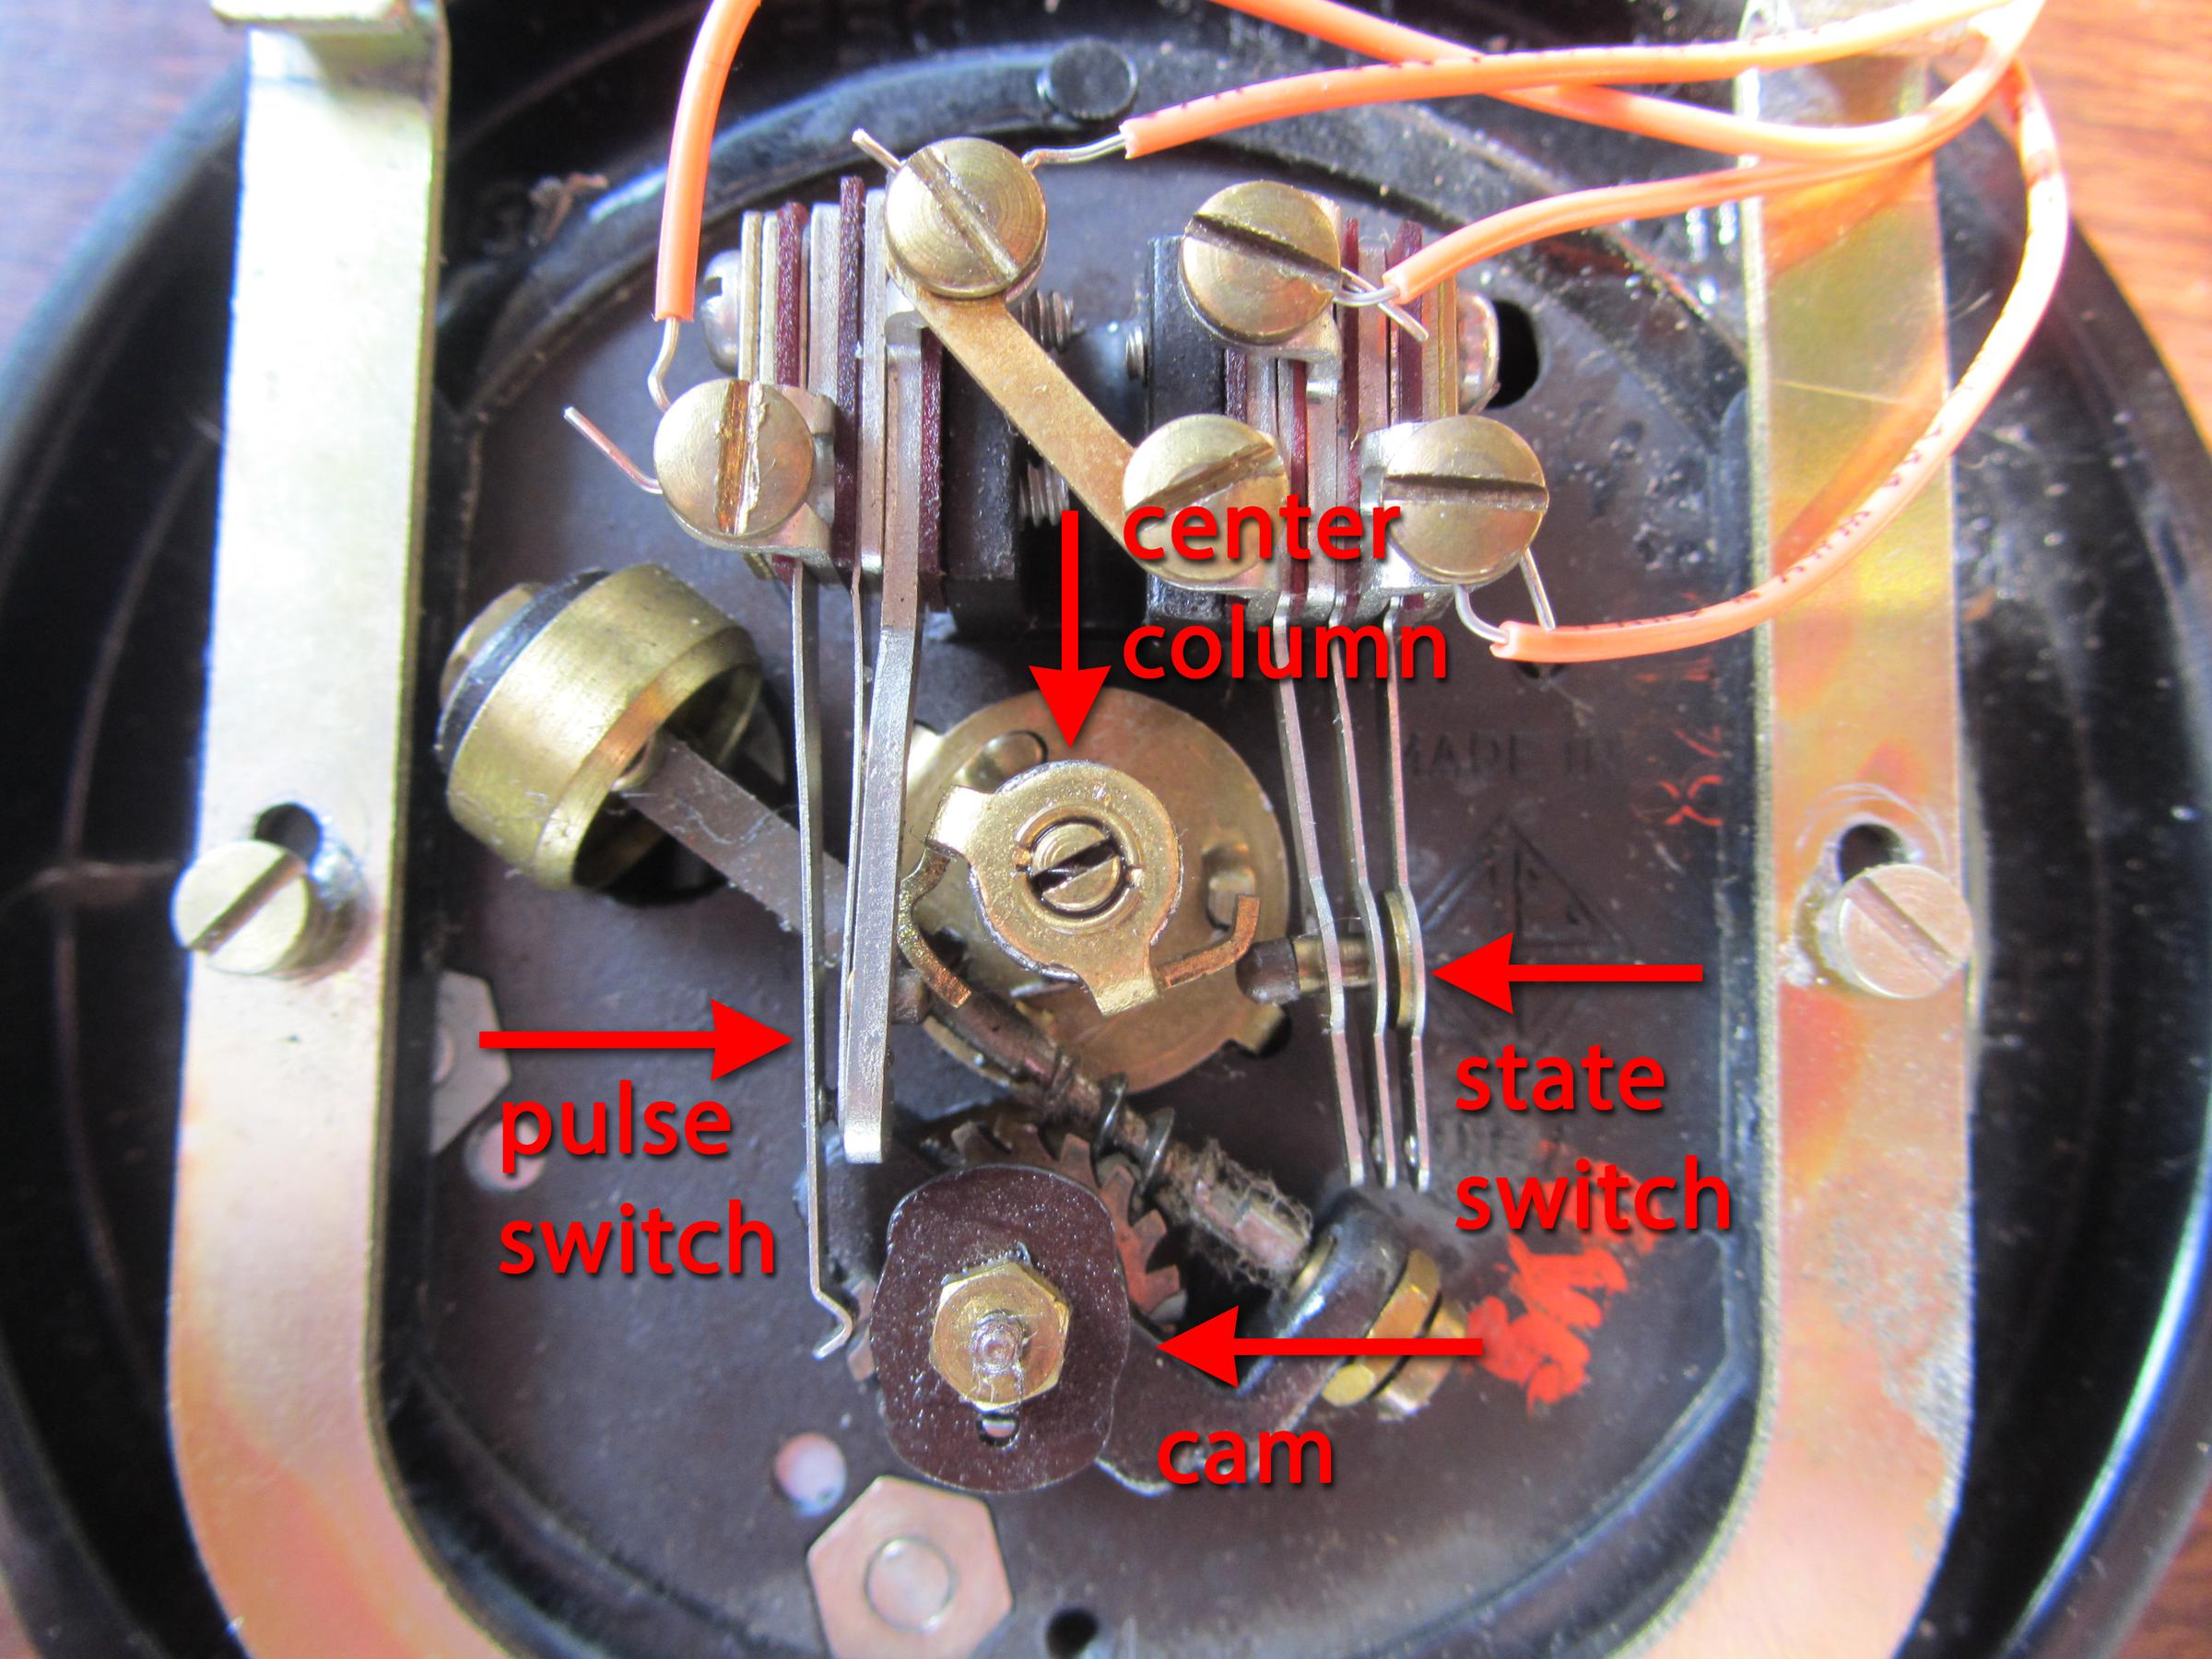
\includegraphics[width=0.6\textwidth, clip=true, trim=200 50 200 70]{images/dialOverview.png}
        \caption{Dial mechanism overview}\label{fig:dialOverview}
    \end{figure}

    The mechanism is shown in Figure~\ref{fig:dialOverview}. While it looks complicated, it's essentially made up of two switches that are toggled by the center column and the cam. When the user releases the dial and it returns to rest, the cam turns, opening and closing the pulse switch to generate the pulse wave. When dialing starts the center column turns counterclockwise, allowing the state switch to close. It stays closed until the dial returns to rest, so it can be used to determine whether a number is being dialed or the dial is at rest. Figure~\ref{fig:dialRest} shows the dial in rest state (pulse switch closed and state switch open), Figure~\ref{fig:dialIsDialing} shows the dial during dialing when no pulse is being generated (pulse switch closed and state switch closed), and Figure~\ref{fig:dialPulse} shows the dial during dialing when a pulse is being generated (pulse switch open and state switch closed).

    We determined which terminals of the dialing mechanism/circuit correspond to which switch, and made a circuit for each switch. We connected one of the Arduino's digital pins in parallel to each of these circuits and enabled the internal pull-up resistors, and we were able to get the state of each switch as a 0 or 1.

    With the ability to sense the state of the switches, we turned to writing the code to detect dialed numbers. The SparkFun project simply counts the number of pulses generated in order to determine which number was dialed, and because this is also the method the telephone exchange uses, it seemed like a logical approach \cite{seidle05}. This method waits for a pulse interval and an inter-pulse interval, and then increments the dialed number, repeating this until the dial comes to rest. However, the SparkFun tutorial notes that ``the dialing doesn't always work,'' and we noticed this as well -- we would sometimes see the Arduino detect a number one off from the actual number dialed. While this happened relatively infrequently for each individual number dialed, it was nearly impossible to dial a 10-digit telephone number correctly. This was, as far as we could tell, a result of difficult-to-tune delays that are necessary to avoid interpreting noise from the switches as a pulse interval or an inter-pulse interval.

    In order to solve this problem, Michael Tingley came up with the idea of using the time it takes the dial to return to rest, rather than the number of pulses, to determine which number was dialed. This method turned out to be extraordinarily reliable. First we looked at the pulse wave on the oscilloscope and determined the length of pulse and inter-pulse intervals: a pulse is approximately 67ms long, and the time between pulses is approximately 42ms. Our implementation is contained in the \verb+getDialedNumber()+ function in our code, so for full details look there, but it works by first determining the time between the first pulse and the dial coming to rest, and then dividing that number by the length of a combined pulse and inter-pulse interval (that is, $67 + 42 = 109$ms). The dial mechanism is consistent enough that simple integer division suffices to very accurately and consistently determine which number was dialed.

    \begin{figure}
        \centering
        \begin{subfigure}[b]{0.32\textwidth}
                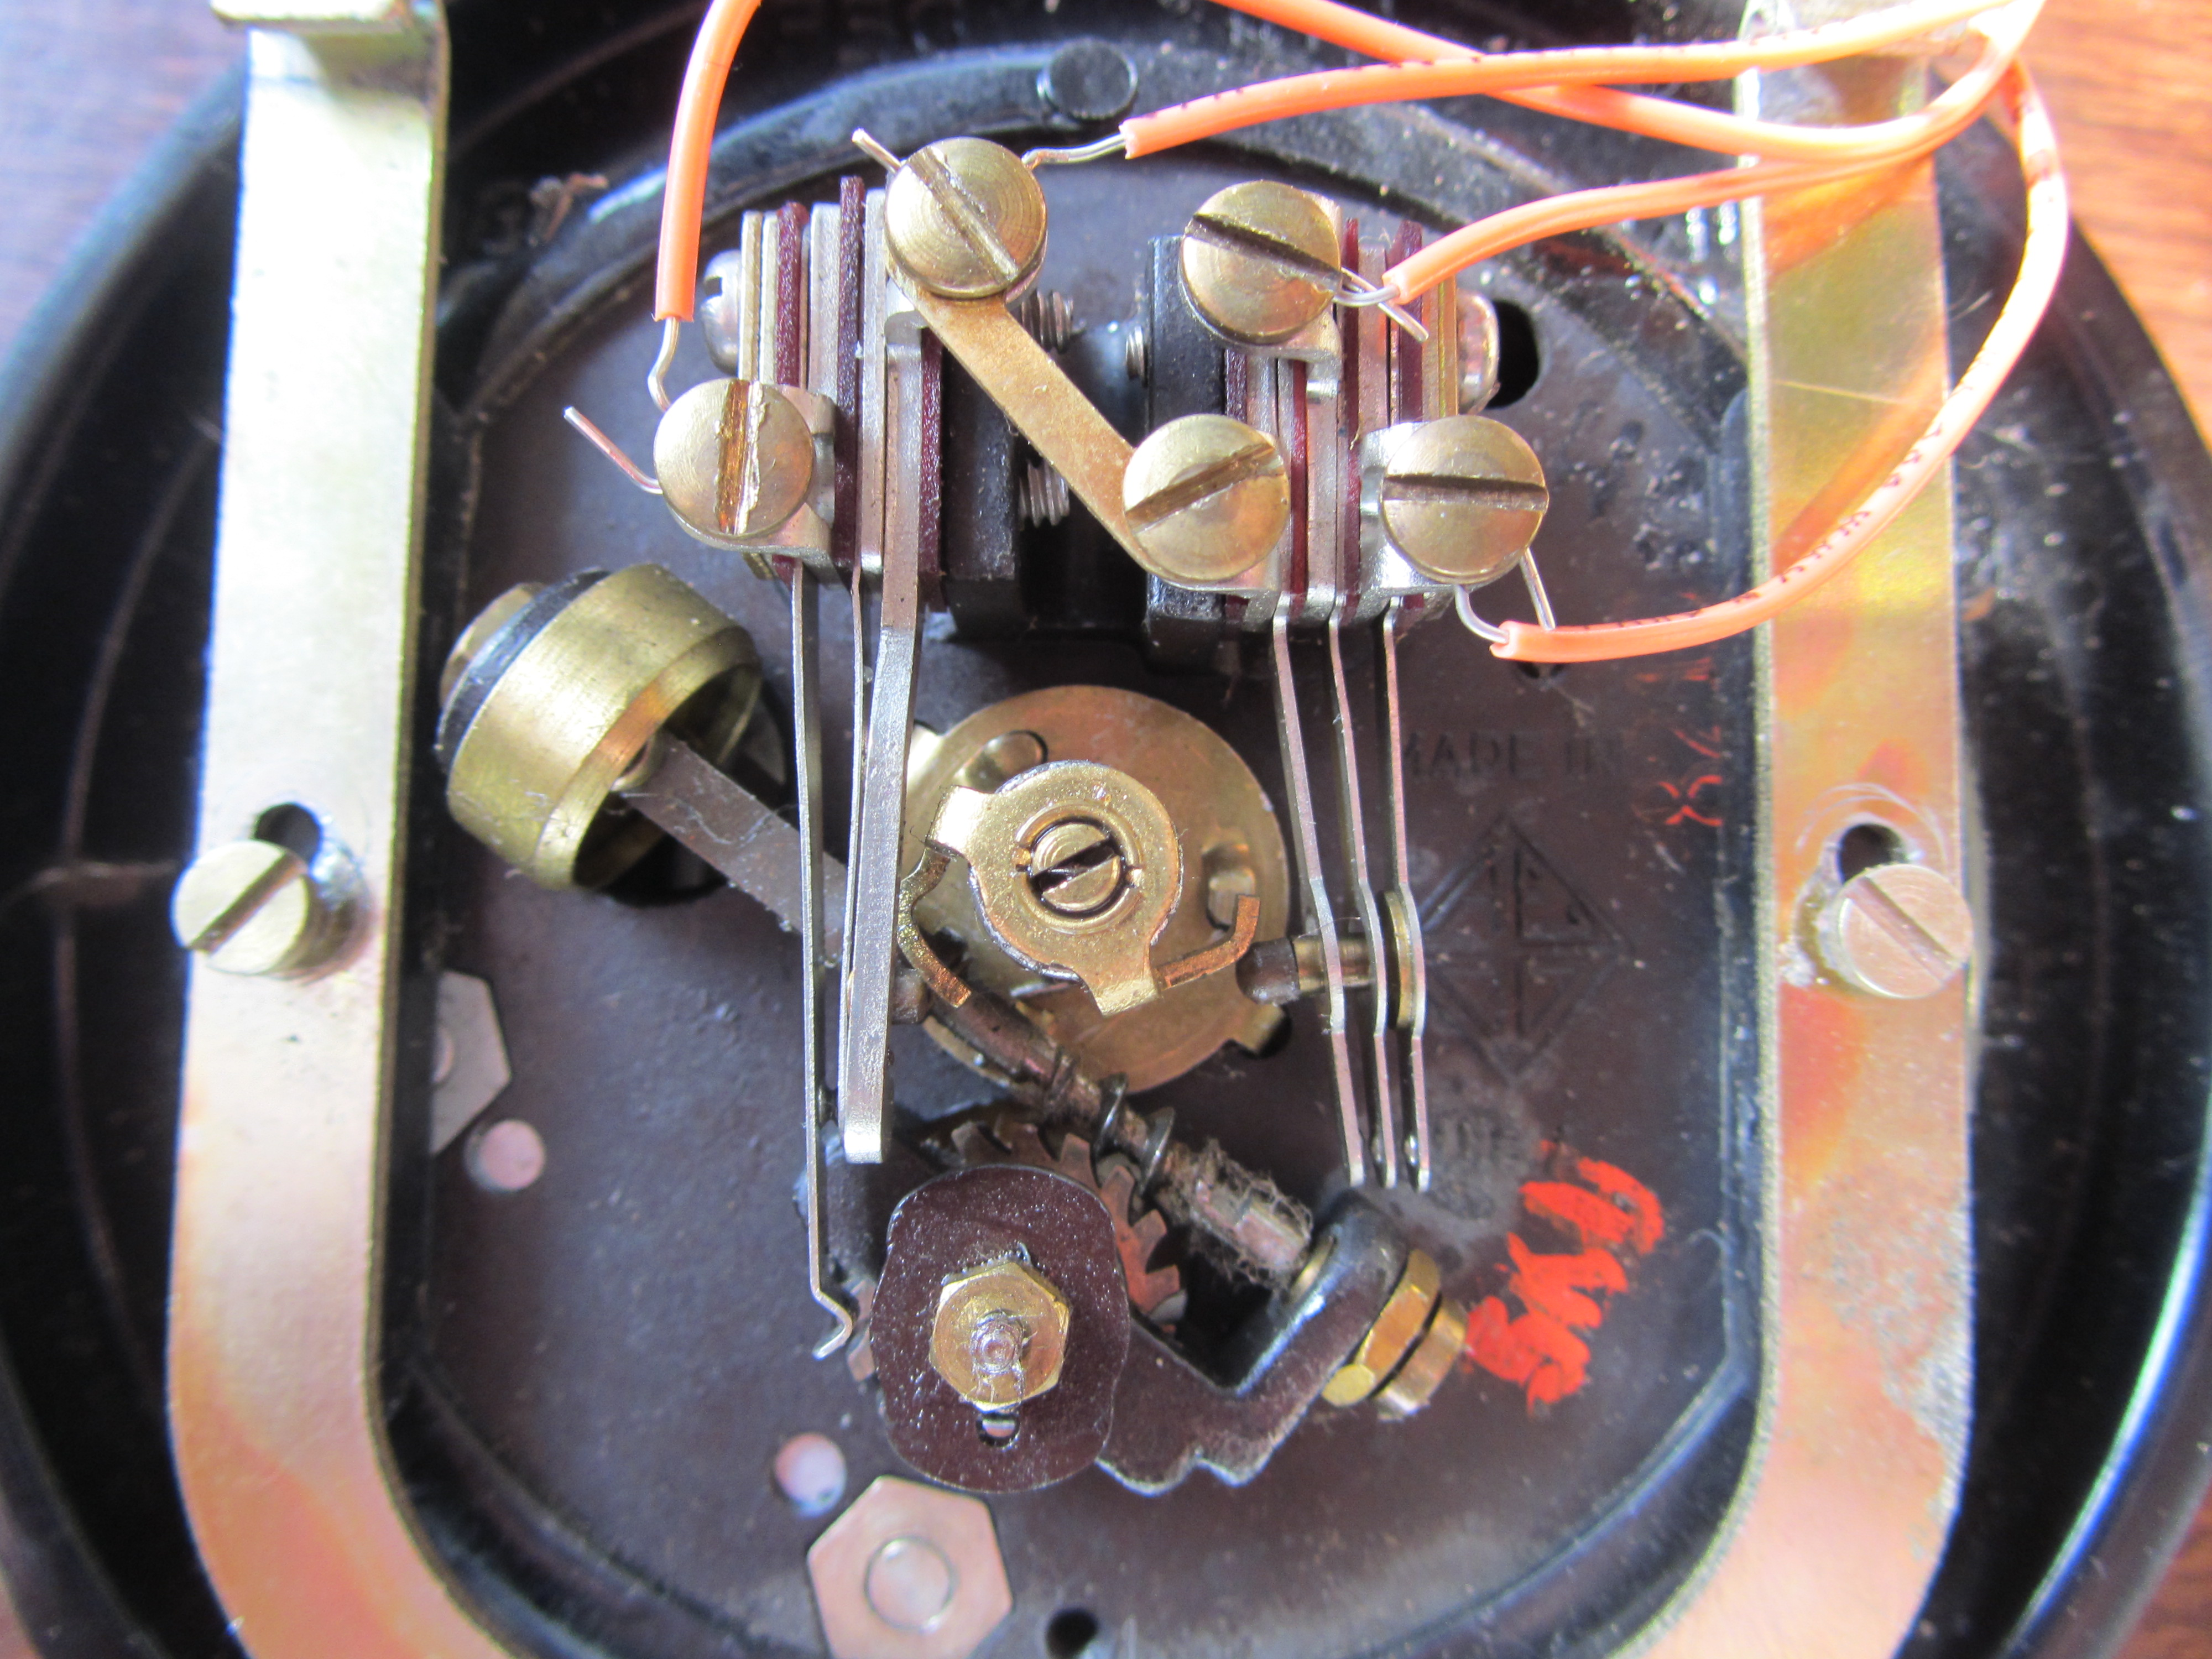
\includegraphics[width=\textwidth, clip=true, trim=300 250 300 70]{images/dialRest}
                \caption{Dial at rest}
                \label{fig:dialRest}
        \end{subfigure}
        %
        \begin{subfigure}[b]{0.32\textwidth}
                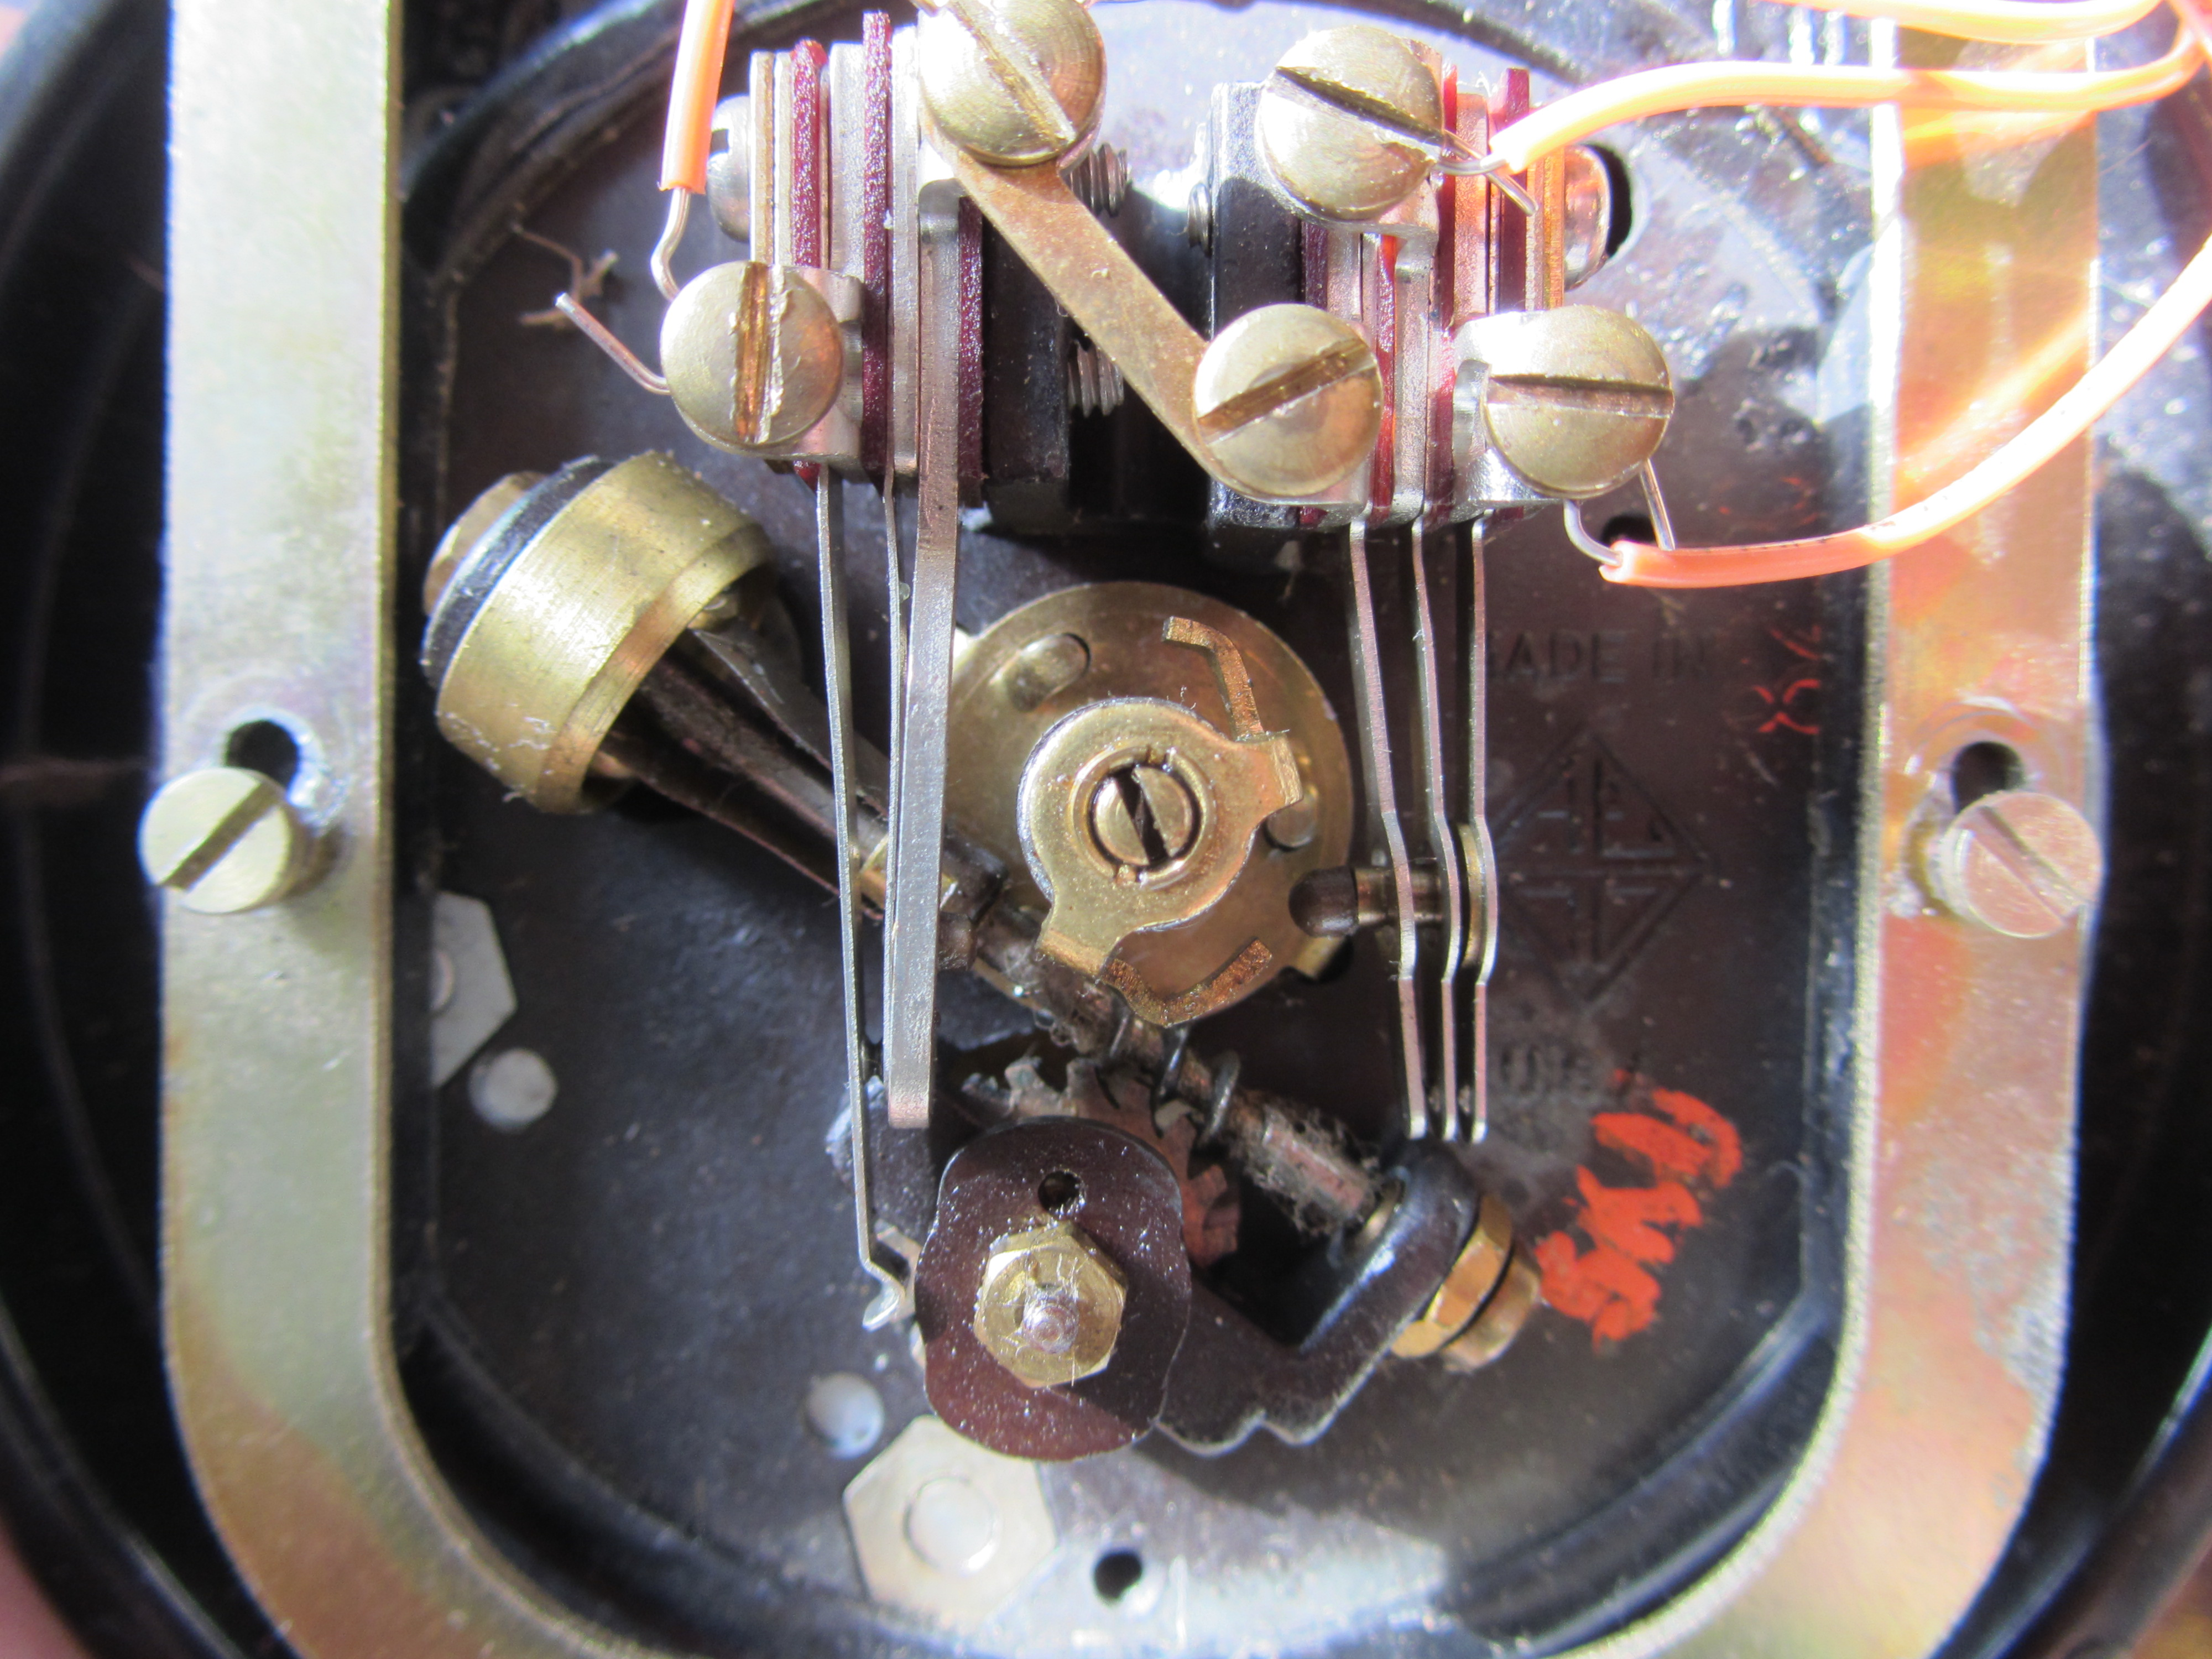
\includegraphics[width=\textwidth, clip=true, trim=300 250 300 70]{images/dialIsDialing}
                \caption{Dialing, pulse closed}
                \label{fig:dialIsDialing}
        \end{subfigure}
        %
        \begin{subfigure}[b]{0.32\textwidth}
                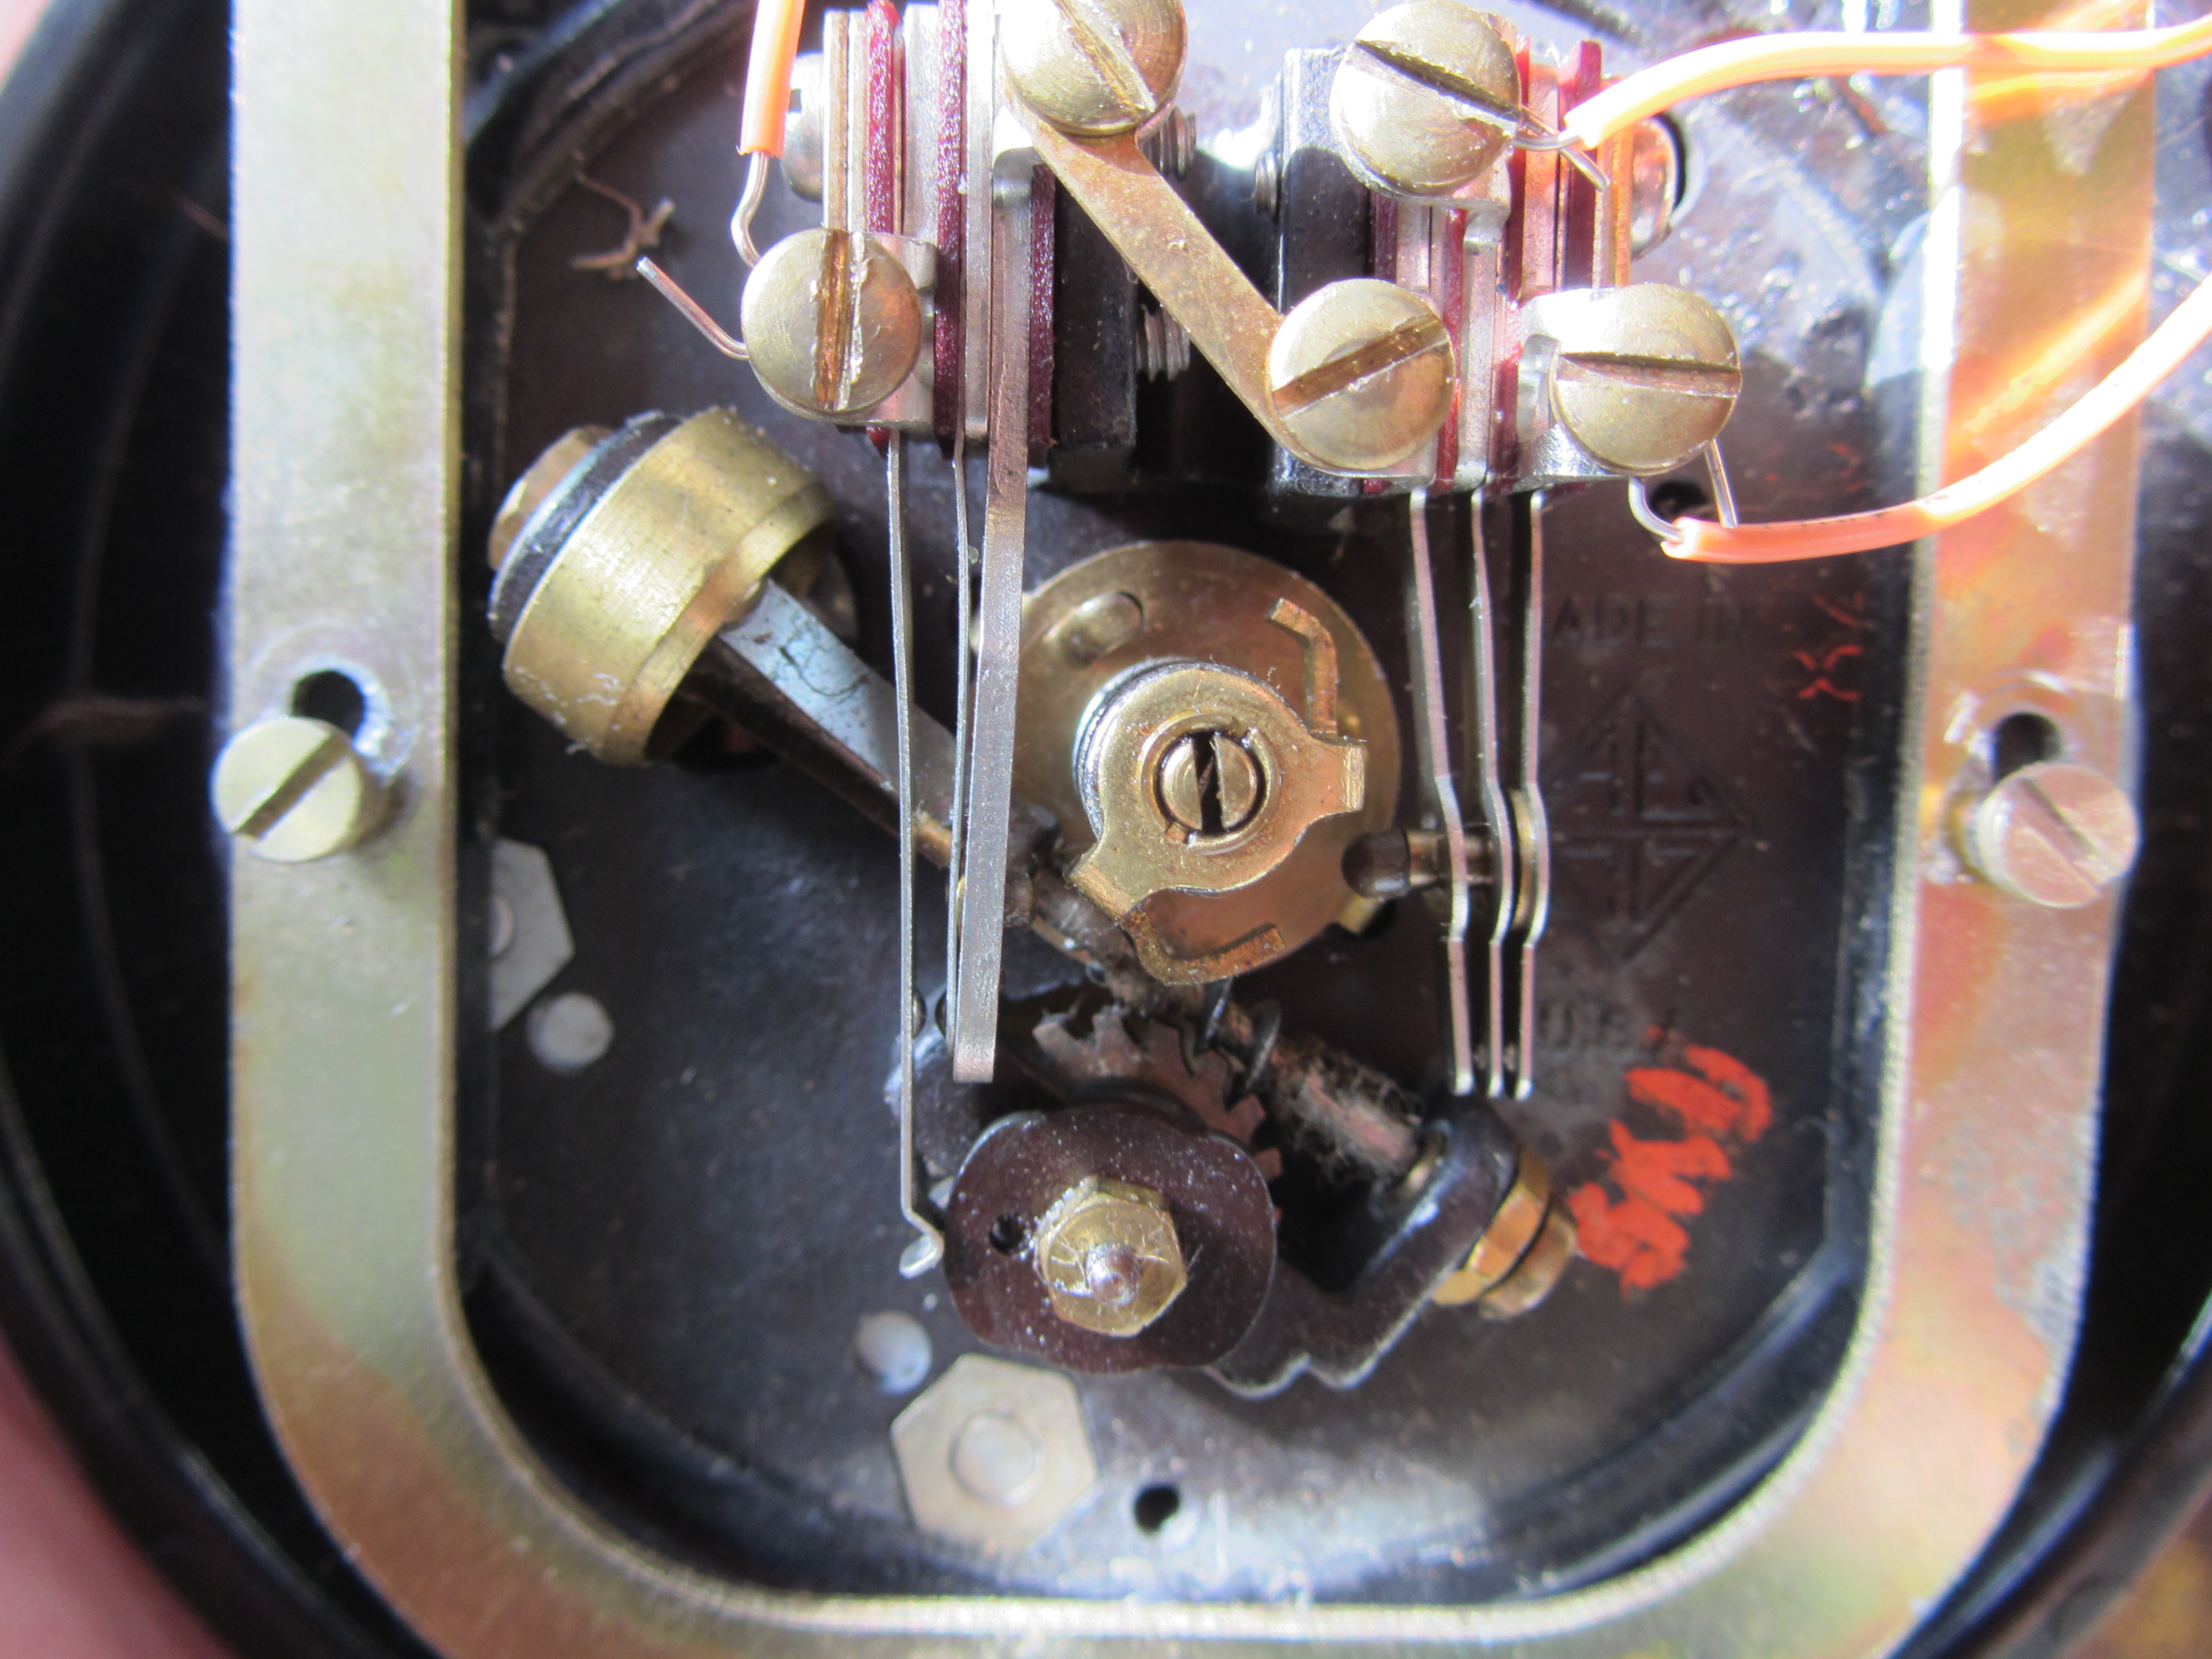
\includegraphics[width=\textwidth, clip=true, trim=300 250 300 70]{images/dialPulse}
                \caption{Dialing, pulse open}
                \label{fig:dialPulse}
        \end{subfigure}
        \caption{Dial switch configurations}\label{fig:dialState}
    \end{figure}

    \subsection{Hacking the Hook Mechanism}
    The third and final piece of information we need to be able to sense is whether the phone is on or off the hook. There are four terminals exposed on the hook switch mechanism, and while these four terminals were connected to the rest of the phone's circuitry, all we need to do is sense which terminals are connected and disconnected when the hook is depressed and released. Some quick trial-and-error lead us to the correct terminals; see Figure~\ref{fig:hookWiring} for details. We built a circuit identical to those used for the dial's switches, connected it to a digit pin on the Arduino, enabled the internal pull-up resistor for the pin, and we were up and running.

    \begin{figure}
        \centering
        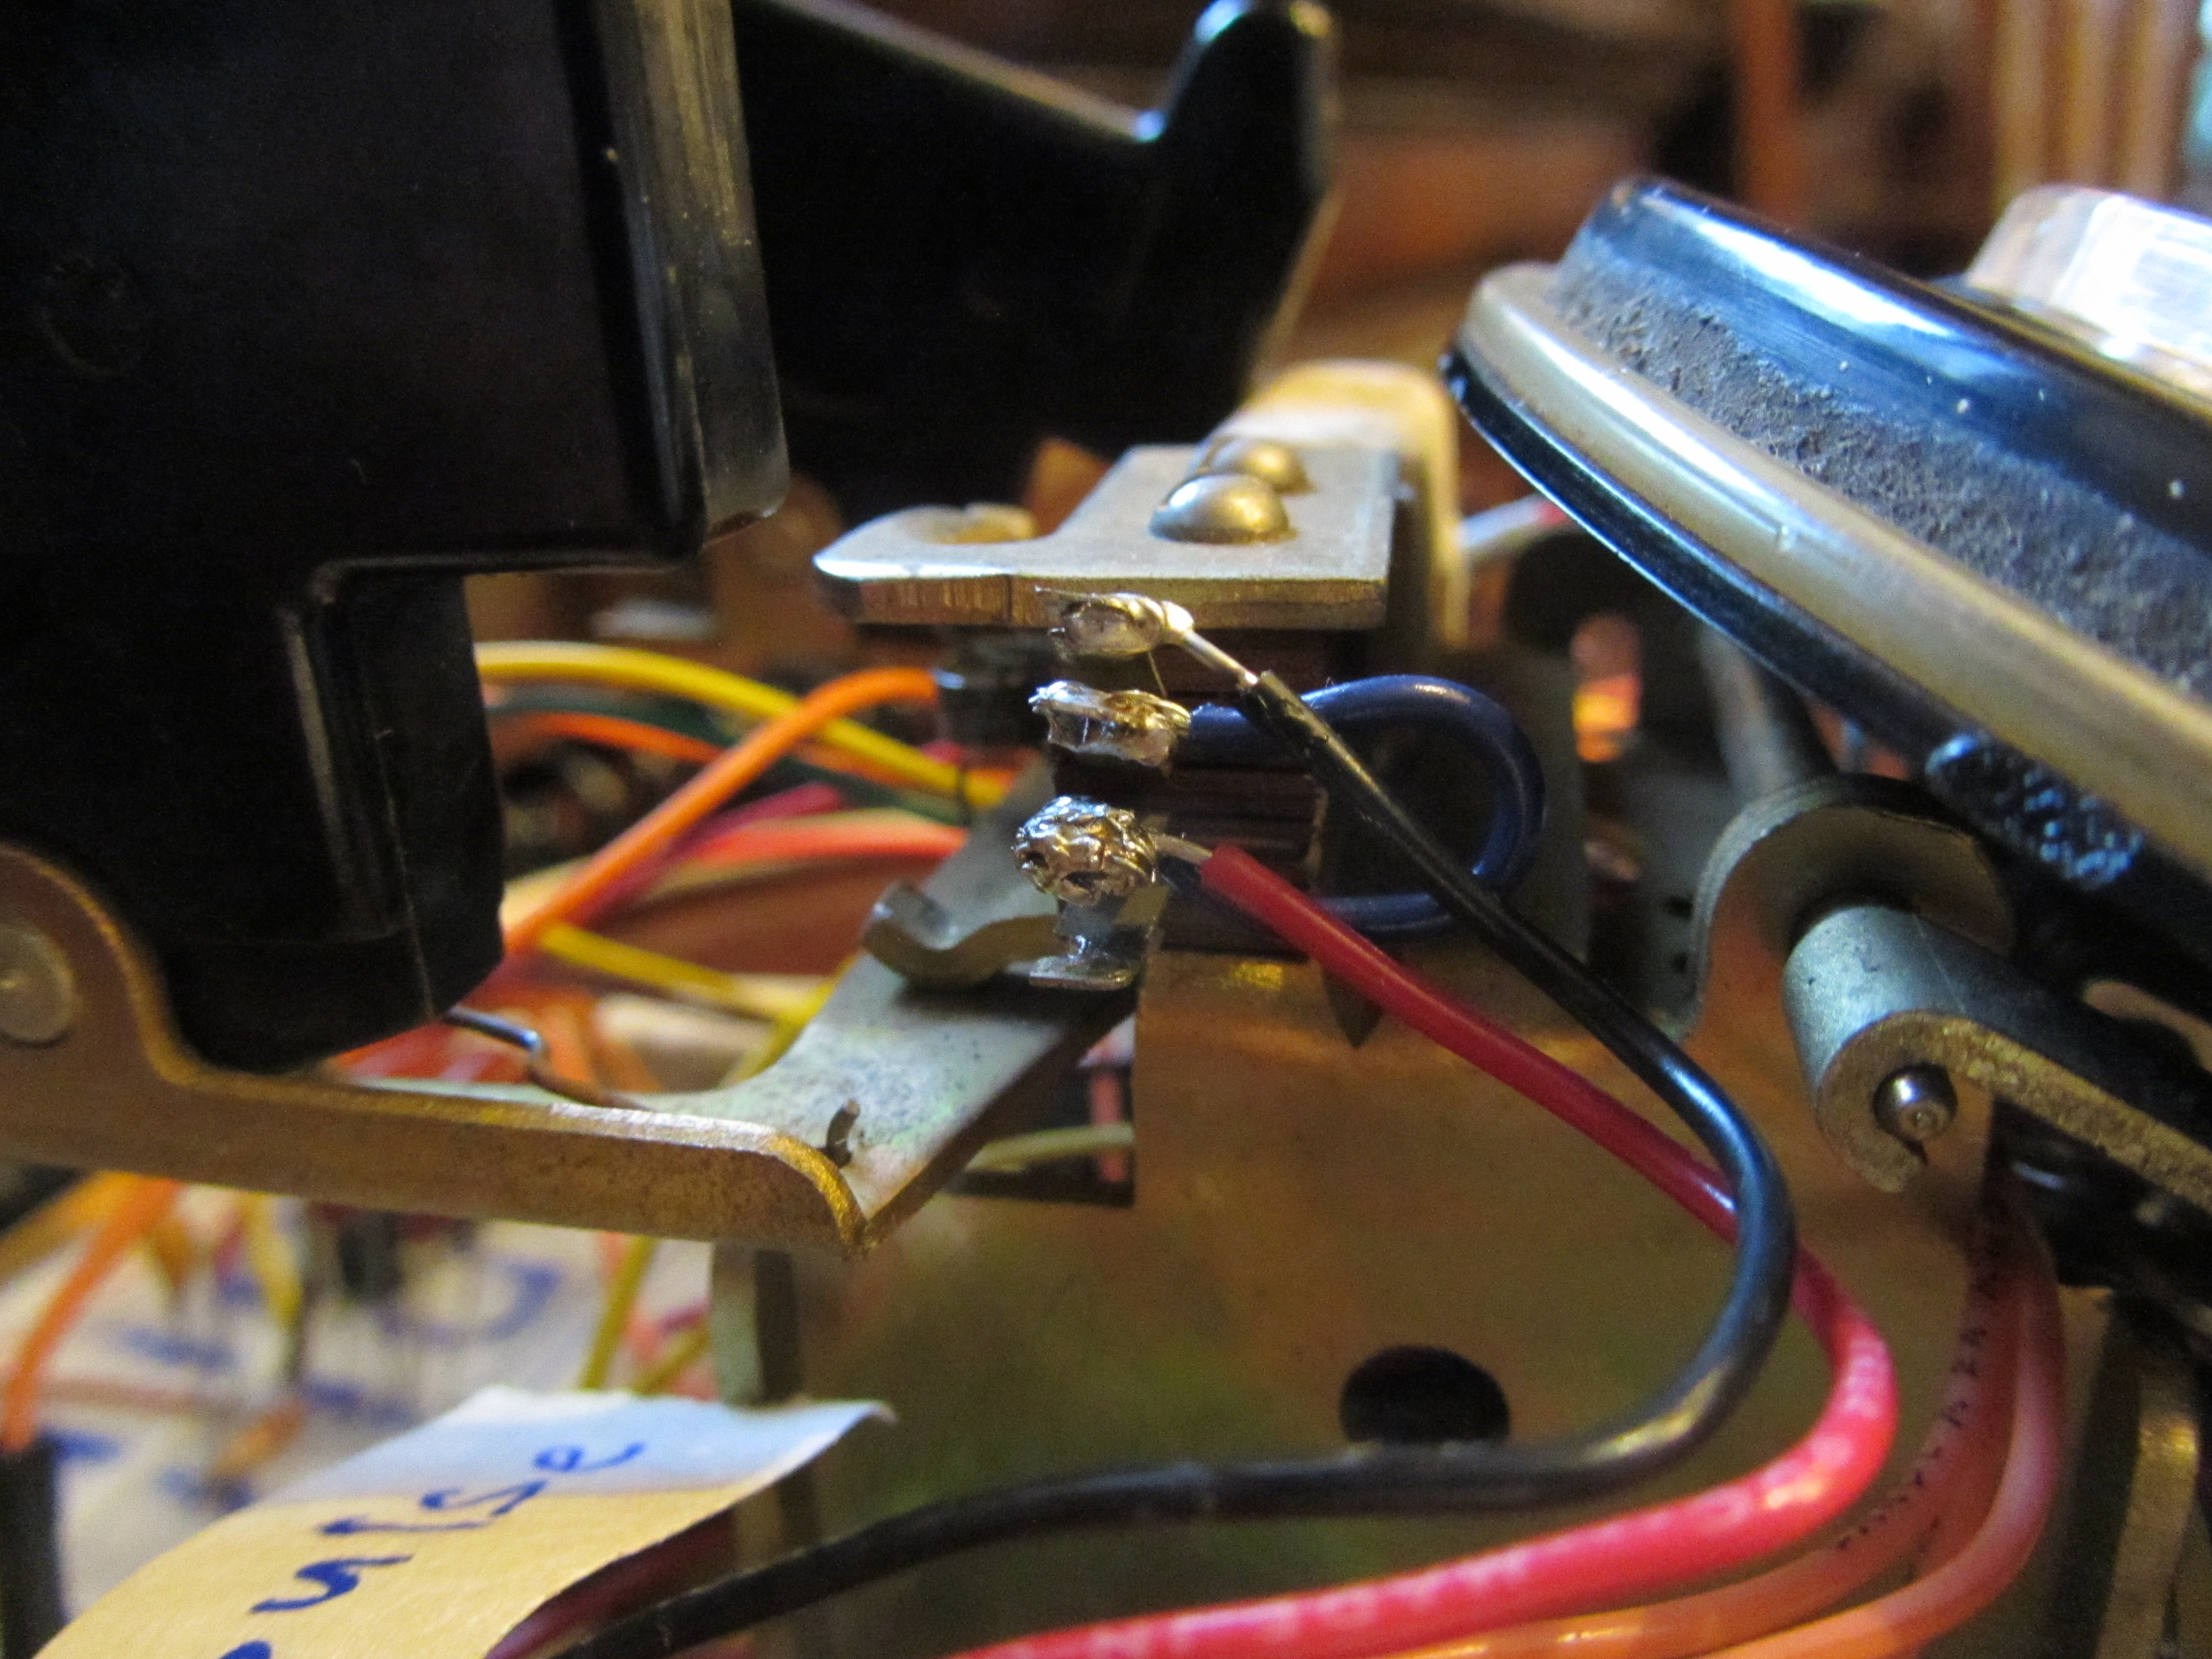
\includegraphics[width=0.6\textwidth, clip=true, trim=200 50 200 70]{images/hookWiring}
        \caption{Hook wiring. When the hook is depressed the circuit made by the red and black wires is completed, and when it is released that circuit is broken.}\label{fig:hookWiring}
    \end{figure}

    \subsection{The Ringer}
    As previously stated, the original ringer requires 80-90V to operate. While SparkFun did build a circuit that can drive the high voltage ringer from a 3.8V source \cite{pete05}, we opted for a lower voltage option for portability, simplicity, and safety. We replaced the original electromagnetic coil and hammer with a small, 18V solenoid. While we did have to remove one of the two bells to mount the solenoid, we were nevertheless able to achieve a sufficiently loud ring reminiscent of, as the good people at SparkFun put it, the  ``classic cardiac arrest twin bell ringer'' of a vintage phone. This also freed up space in the phone for our other components.

    Because the Arduino operates at 5V and the solenoid requires 18V, we built a simple circuit with a relay to activate the solenoid using the output of one of the Arduino's digital pins. Kyle wrote code to activate the solenoid in bursts while ringing to make it sound more authentic. Check out our video to hear it!

    \begin{figure}
        \centering
        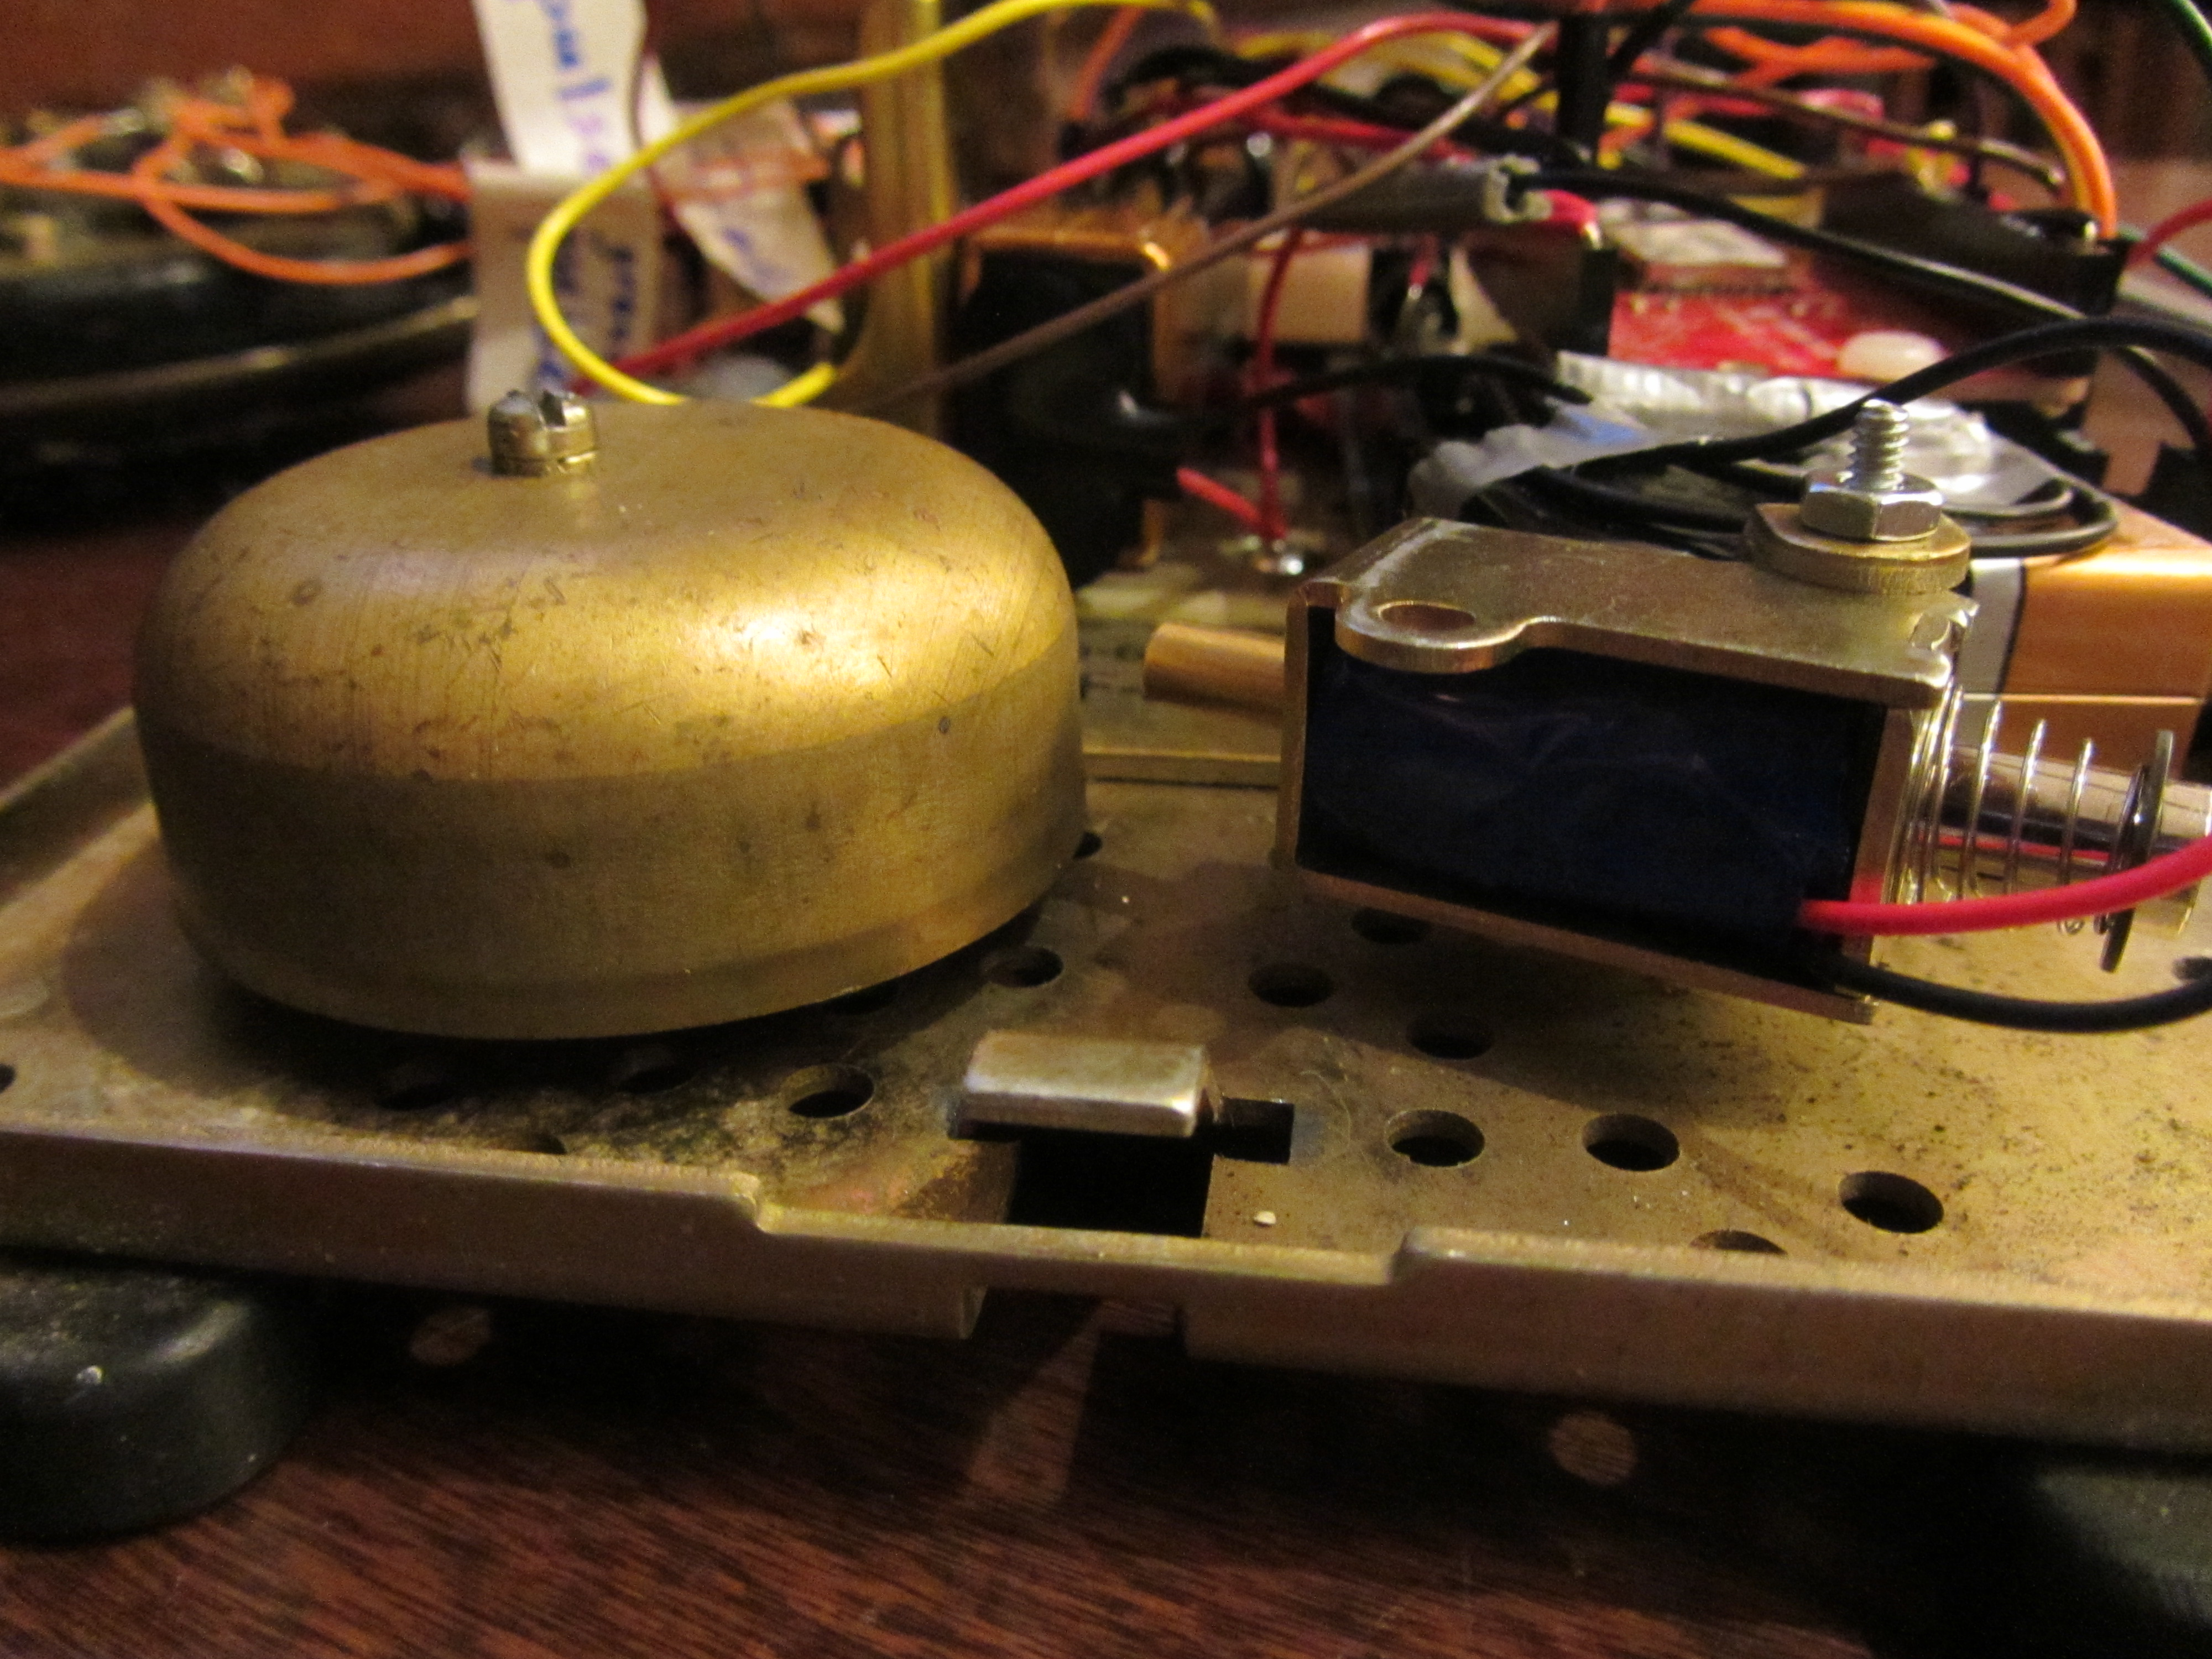
\includegraphics[width=0.6\textwidth, clip=true, trim=0 450 0 0]{images/solenoidMount}
        \caption{Ringer solenoid mount.}\label{fig:solenoidMount}
    \end{figure}

    \subsection{Interfacing the Arduino and the Bluetooth Module}
    We used the RN-52 Bluetooth audio module from Roving Networks. The datasheet is at \cite{rn52Datasheet} and the command reference is at \cite{rn52CommandRef}. The module handles audio input and output, so we don't need to handle that on the Arduino. What we do need to is as follows:

    \begin{itemize}
        \item Listen for events from the Bluetooth module. Most importantly, we listen for the event that signifies an incoming call. The RN-52 brings one of its pins low when an event occurs, so we continuously read from this pin in the Arduino \verb+loop+ to detect when an event occurs.
        \item Accept and end calls when the handset is picked up and hung up, respectively.
        \item Make a call when the user finishes dialing a number.
    \end{itemize}

    The RN-52 exposes a set of ASCII commands that can do all of this quite easily, so all we need to do is send ASCII strings terminated with \verb+\r+ to the RN-52 over its UART serial interface to control it. Take a look at the module's command reference (\cite{rn52CommandRef}) and our code for examples.

    The one issue with serial communication between the Arduino and the RN-52 is voltage levels -- the Arduino Uno uses 5V logic, but the RN-52 uses 3.3V logic. In order to interface the two, we used a simple voltage divider to bring the Arduino's 5V transmit line down to 3.3V before connecting it to the RN-52's receive pin. We then built a 3.3V to 5V voltage level converter circuit to bring the RN-52's 3.3V transmit line up to 5V before connecting it to the Arduino's receive pin \cite{hobbytronics14}, but we discovered that this is not actually necessary -- 3.3V is high enough for the Arduino to accurately receive data from the RN-52. So, for compactness of our final circuit, we omitted the voltage level converter. However, it would likely be a good idea to include real voltage level converters on both serial communication lines in a production version of the circuit to make it as robust as possible.

    \subsection{Audio}
    The final piece of the original phone hardware we needed to integrate was the handset. We started with the speaker. The RN-52's datasheet states that it has a built-in amplifier suitable for driving $16\Omega$ speakers \cite{rn52Datasheet}, and even though the handset's speaker tested at $40\Omega$, we hooked it up to the RN-52's audio output pins to give it a try. We played some music over the Bluetooth connection, and it came through loud and clear with surprising clarity. Sweet!

    The microphone took a lot more work. We were able to successfully bias it with a standard microphone biasing circuit and record clear, reasonably good quality audio on a computer, but integrating it with the Bluetooth module was much harder. The first problem is that the handset has only three wires: the speaker and microphone each have a wire directly to them, and the third wire is shared. We tried hooking up the microphone directly to the Bluetooth module, and while we were able to pick up audio, the volume was low and there was some nasty echo due to the shared wire. We then tried to properly bias the microphone, and while the input became louder, voices became unintelligible. However, the RN-52's datasheet contains a set of circuit diagrams labeled ``Typical Application Schematic,'' which includes an audio input circuit \cite{rn52Datasheet}. We built the circuit, and, unsurprisingly, it worked. The audio quality isn't phenomenal, but given the very old hardware, it's passable. We also don't filter the signal to remove noise or background interference, which would likely improve the quality significantly and would be a good addition for a future version of this project.

    \subsection{The Code}
    TODO

    \subsection{Circuit Consolidation and Mounting}
    TODO

    \section{Team Management}
        We all worked collaboratively on most parts of the project. We all came into the project with similar background; all of us are computer science majors that are generally comfortable with coding but not very comfortable with the hardware side of the project. Nonetheless, there were a few areas of specialization that each member took responsibility for.

        \begin{description}
            \item[Dial pulses and handset]
                Michael Traver was responsible for a lot of the hardware wiring. He worked on figuring out where each wire should be attached in order to sense a dial pulse or to sense the state of the handset (on the hook/off the hook). Michael Tingley improved the code for pulse sensing. Instead of sensing each pulse individually, he came up with the algorithm to listen for the `length' of the input to determine which number was dialed, which proved to be more accurate.
            \item[The ringer]
                Michael Tingley was responsible for much of the work with the ringer. He was responsible for early prototyping of a ringer and for designing the relay circuit to fire the solenoid. Kyle Solan was responsible for the engineering that went into the final ringer. Kyle modified the original ringer and mounted the new one, and configured the solenoid and tweaked the code in order to produce a sound that could be convincing for a 1940s-style ring.
            \item[Microphone and speaker]
                Kyle and Traver did most of the work on the microphone and ringer. Traver worked diligently to reduce echo and increase volume of the microphone. Kyle was responsible for speaker output. Both worked on figuring out how mic biasing works (e.g., what configuration of capacitors to use), and how to correctly ground the circuit. (We had some issues with grounding the circuit because both the speaker and the microphone used the same cable for grounding.)
            \item[Bluetooth module]
                Everyone on the team worked on the bluetooth module. This was easily the hardest part of the project. We had issues soldering, using the correct voltages and baud rates, providing the correct power, and reading the output using the correct encoding. It's difficult to break down each challenge by who solved it, since we all pooled our brainpower when trying to decipher cryptic tutorials online or debugging the circuits with the oscilloscope and multimeter.
            \item[Changing voltages]
                Throughout working with the bluetooth module, we found out that it only accepted/output 3.3V signals. Since the Arduino worked with 5V signals, this turned out to be a problem. Tingley and Traver worked on rigging up circuits to fix this. To convert 5V to 3.3V, we were able to use a simple voltage divider. However, to convert 3.3V to 5V, we had to use a more complex setup of transistors and a 5V input bias. (In the end, the Arduino turned out to be sensitive enough to 3.3V as opposed to 5V, and so we were able to exclude this circuit in the final project.)
            \item[Circuit reduction, portability]
                Traver and Kyle worked on making the circuit smaller and more portable. This involved condensing everything from 3 long circuit boards to a single short one. In addition, they worked on trimming wires as appropriate and carefully compacting everything inside of the phone case so that the device could be made portable. All three of us worked on wiring up the circuit with batteries and making it portable!
        \end{description}

    \section{Outlook and Possible Improvements}
        \begin{description}
            \setlength{\parskip}{2mm}
            \item[LCD display]
                We accomplished all of our major objectives and finished most of our reach goals. The one main thing that we would do with additional time is to use an LCD display to display useful information for the user.

                One of the things that we would like to do is to use  the LCD to display numbers that the user has dialed so far during a dialing sequence. We found that it is very disorienting to dial a number on an old rotary phone. Since you have to wait several seconds between entering numbers, it is very easy to forget where you were. Furthermore, since we read numbers using analog circuitry, it would be useful to get visual feedback that the number was interpreted correctly.

                Additionally, we would like to be able to use the LCD to display caller information. It would be relatively easy to display the incoming number. If possible, we would also like to use the LCD to display the caller's name, using the phonebook in the bluetooth-linked phone. However, this appears to be very difficult, and would require custom phone querying using the data pipe mode on the bluetooth module.
            \item[Improving audio input]
                The audio quality from the phone's original microphone isn't great. Filtering the audio signal to remove background noise and signal noise would improve usability a great deal. While we were excited that we were able to get the phone working with the original microphone because we wanted to preserve as much of the original hardware as possible, replacing the microphone with a modern one may be warranted if the quality cannot be improved sufficiently.
            \item[Texting mode]
                Assuming we care nothing at all about usability, we would like to include a texting mode. This would be virtually unusable, but the basic idea is that you lift the handset up and wait 10 seconds until you hear a beep from the phone. Then you're in texting mode. You can enter letters using a T9-style input method (if we have the LCD, that can show letters already entered). To enter a letter, you simply wait a number of seconds between entries and the letter will automatically be entered. To send the text, you would put the handset down, and then dial the number to send the text to.

                If we have the LCD, we could even display received text messages on it. Because why not.
        \end{description}

    \section{Acknowledgments}
        We would like to thank John the TF, as we ``accidentally'' insulted his field of study both verbally and metaphorically multiple times throughout this class and final project. Kyle would like to thank the course staff for making available so many Arduinos, as at one point in time we used 10 Arduinos and thought we broke a few of them. Traver would like to thank SparkFun for providing a literally infinite number of tutorials on how to launch objects of assorted sizes using various mechanisma. Tingley would like to thank Traver for having such a fantastic first name. Finally, we would like to thank the 1940s. As without them, we would not physically exist at this present point in time.

    \section{Disclaimer}
        It is okay with us to share our report, code that we wrote, and photos and videos of our product.

    \appendix
    \section{Appendix}
    TODO

    \newpage
    \bibliographystyle{plain}
    \bibliography{es50report}

\end{document}
